\documentclass[12pt,a4paper]{article}

\usepackage{fullpage}

\usepackage{pdfpages}

\begin{document}

\pagestyle{empty}

\begin{center}

\begin{large}

\mbox{}
\vspace{4cm}

\begin{LARGE}
Proceedings of the \\
International Workshop \& Tutorial on \\

\bigskip

\textbf{Adaptive Text Extraction and Mining}

\bigskip

held in conjunction with the 
14th European Conference on Machine Learning 
and the
7th European Conference on Principles and Practice of Knowledge Discovery in Databases
\end{LARGE}

\bigskip
\mbox{}
\bigskip

22 September 2003 \\
Cavtat--Dubrovnik (Croatia) 

\bigskip

\begin{verbatim}
              www.dcs.shef.ac.uk/~fabio/ATEM03
\end{verbatim}

\bigskip
\mbox{}
\bigskip

\textbf{Organizing Committee:} \\
Fabio Ciravenga (University of Sheffield, UK) \\
Nicholas Kushmerick (University College Dublin, Ireland)

\end{large}
\end{center}

\newpage

\begin{center}

\mbox{}
\vspace{2cm}

\begin{large}
\textbf{Table of Contents}
\end{large}

\mbox{}
\bigskip
\mbox{}
\bigskip
\mbox{}

\begin{tabular}{p{0.9\textwidth}r}

Preface
& 1 \\

Exploiting the feature vector model for learning linguistic representations of relational concepts
\emph{(Roberto Basili, Maria Teresa Pazienza, Fabio Massimo Zanzotto)}
& 2 \\

\mbox{} \\[-8pt]

Automatic acquisition of taxonomies from text: FCA meets NLP
\emph{(Philipp Cimiano, Steffen Staab, Julien Tane)}
& 10 \\

\mbox{} \\[-8pt]

Active learning selection strategies for information extraction
\emph{(Aidan Finn, Nicholas Kushmerick)}
& 18 \\

\mbox{} \\[-8pt]

Active learning for information extraction with multiple view feature sets
\emph{(Rosie Jones, Rayid Ghani, Tom Mitchell, Ellen Riloff)}
& 26 \\

\mbox{} \\[-8pt]

Information extraction from multi-document threads
\emph{(David Masterson, Nicholas Kushmerick)}
& 34 \\

\mbox{} \\[-8pt]

An analysis of ontology-based query expansion strategies
\emph{(Roberto Navigli, Paola Velardi)}
& 42 \\

\mbox{} \\[-8pt]

Combining ontological knowledge and wrapper induction techniques into an e-retail system
\emph{(Maria Teresa Pazienza, Armando Stellato, Michele Vindigni)}
& 50 \\

\mbox{} \\[-8pt]

Meta-learning beyond classification: A framework for information extraction from the Web
\emph{(Georgios Sigletos, Georgios Paliouras, Constantine D. Spyropoulos, Takis Stamatopoulos)}
& 58 \\

\mbox{} \\[-8pt]

Information extraction via double classification
\emph{(An De Sitter, Walter Daelemans)}
& 66 \\

\mbox{} \\[-8pt]

Information extraction as a Semantic Web technology: Requirements and promises
\emph{(Mark Stevenson, Fabio Ciravegna)}
& 74 \\

\mbox{} \\[-8pt]

Finding educational resources on the Web: Exploiting automatic extraction of metadata
\emph{(Cynthia Thompson, Joseph Smarr, Huy Nguyen, Christopher Manning)}
& 79 \\

\mbox{} \\[-8pt]

Semantic relations in concept-based cross-language medical information retrieval
\emph{(\v{S}pela Vintar, Paul Buitelaar, Martin Volk)}
& 83 \\

\mbox{} \\[-8pt]

Tutorial Notes
\emph{(Fabio Ciravenga, Nicholas Kushmerick)}
& 92

\end{tabular}

\end{center}

\newpage

\setcounter{page}{1}
\pagestyle{plain}

\begin{center}
\large Preface
\end{center}

\medskip

\begin{small}

\noindent Vast quantities of valuable knowledge are embedded in
unstructured textual formats. Peta\-bytes of text are currently
available on the public Web, in intranets and other private
repositories, and on our personal desktop machines. In many cases, the
only way to access such documents is through blunt instruments such as
keyword-based document retrieval. In recent years, there has been
significant research (and considerable commercial) interest in
technologies for automatically extracting and mining useful structured
knowledge from unstructured text. Current trends suggest a movement
away from pure natural language processing approaches requiring the
manual development of rules, to shallower, less knowledge-intensive
approaches based on techniques from machine learning, information
retrieval and data mining.

Adaptive text extraction and mining is an enabling technology with a
wide variety of applications. On the Web, automated knowledge capture
from text would open the way for both better retrieval, and advanced
business applications (e.g. B2B/B2C applications mediated by
knowledge-aware agents). For knowledge management, capturing the
knowledge contained in a company's repositories would encourage
knowledge to be shares and reused among employees, improving
efficiency and competitiveness. Extracting information from texts is
an important step in capturing knowledge, e.g. for populating
databases or ontologies, supporting document annotation (e.g. for the
Semantic Web), for learning ontologies, etc.

Following the tradition of the previous workshops on the same topic
held at AAAI-1998 (www.isi.edu/info-agents/RISE/ML4IE), \ \ ECAI-2000
(www.dcs.shef.ac.uk/\verb|~|fabio/Local/\-ecai- work\-shop.\-html), and
IJCAI-2001 (www.smi.ucd.ie/ATEM2001), ATEM-03 will bring together
researchers and practitioners from different communities (e.g. machine
learning, text mining, natural language processing, information
extraction, information retrieval, ontology learning), to discuss
recent results and trends in mining texts for knowledge capture.

The program includes two types of submissions: nine long papers
describing completed research, and three short papers describing
ongoing work or challenging ideas. Ten papers come from Europe
(Belgium, Germany, Greece, Italy, Ireland, United Kingdom), two come
from USA.  Each paper was reviewed by at least two
reviewers. Acceptance rate was 46\% (12 out of 26).

A short tutorial is associated with the workshop, providing an
introduction to Information Extraction from Web Documents.  This
tutorial follows on an earlier successful tutorial at the European
Conference on Artificial Intelligence in 2002 in Nantes.

We thank the reviewers for their cooperation in the reviewing process,
especially considering that the large number of submissions caused a
heavier load than expected.  The Programme Committe was comprised of:

\begin{center}
\begin{tabbing}
xxxxxxxxxxxxxx\=xxxxxxxxxxxxxxxxxxxxxx\=\kill
\>Christopher Brewster\>University of Sheffield, UK \\
\>Joe Carthy\>University College Dublin, Ireland \\
\>Philipp Cimian\>University of Karlsruhe, Germany \\
\>Valter Crescenzi\>Universit\a`{a} di Roma Tre, Italy \\
\>An De Sitter\>University of Antwerp, Belgium \\
\>Dayne Freitag\>Fair Isaac Corporation, USA \\
\>Rayid Ghani\>Accenture Technology Labs, USA \\
\>Rosie Jones\>Accenture Technology Labs, USA \\
\>Christopher Manning\>Stanford University, USA \\
\>Ion Muslea\>SRI International, USA \\
\>Hwee Tou Ng\>National University of Singapore, Singapore \\
\>Horacio Saggion\>University of Sheffield, UK \\
\>Mark Stevenson\>University of Sheffield, UK
\end{tabbing}
\end{center}

\end{small}

\newpage

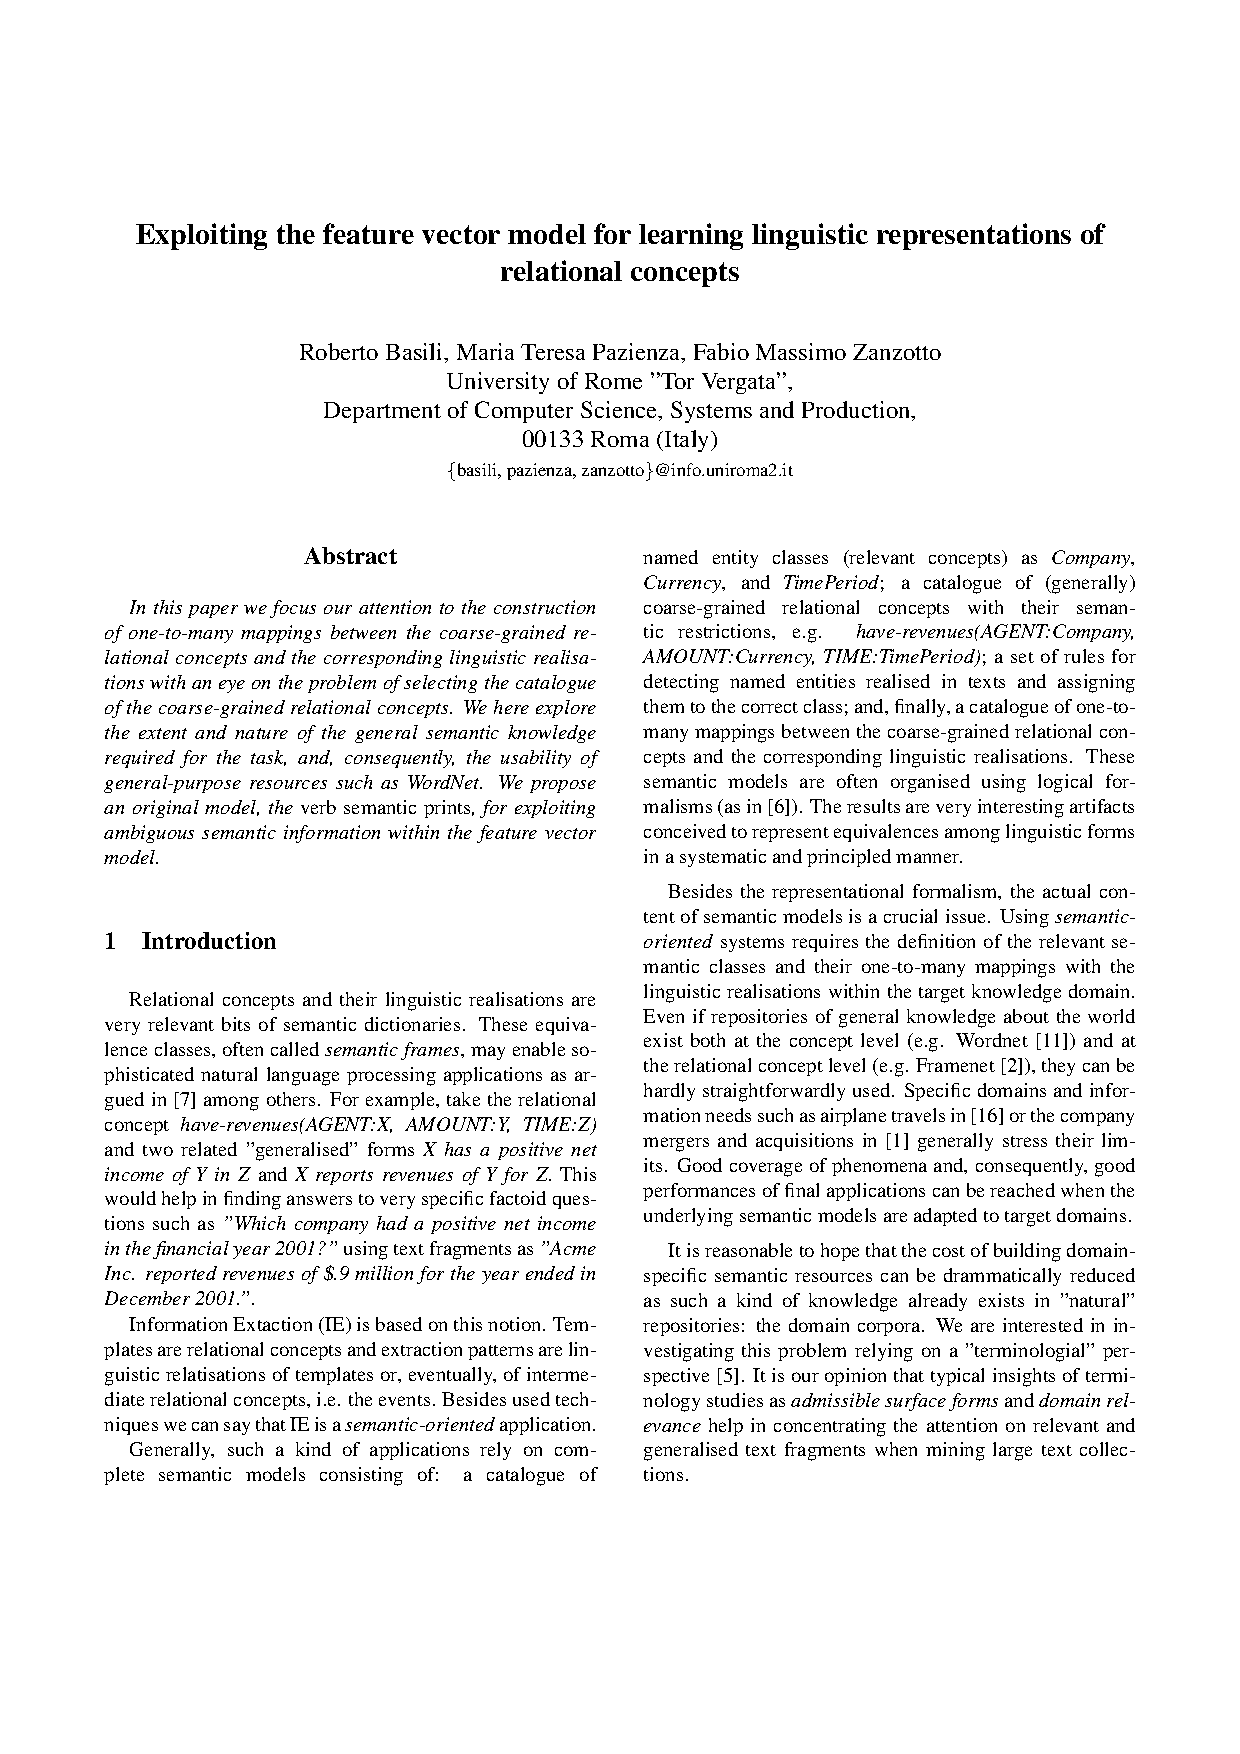
\includepdf[trim= 0 100 0 0,clip=true,offset=0 25,pagecommand={\mbox{}},pages={1-8}]{basili-ecml03-atem.pdf}
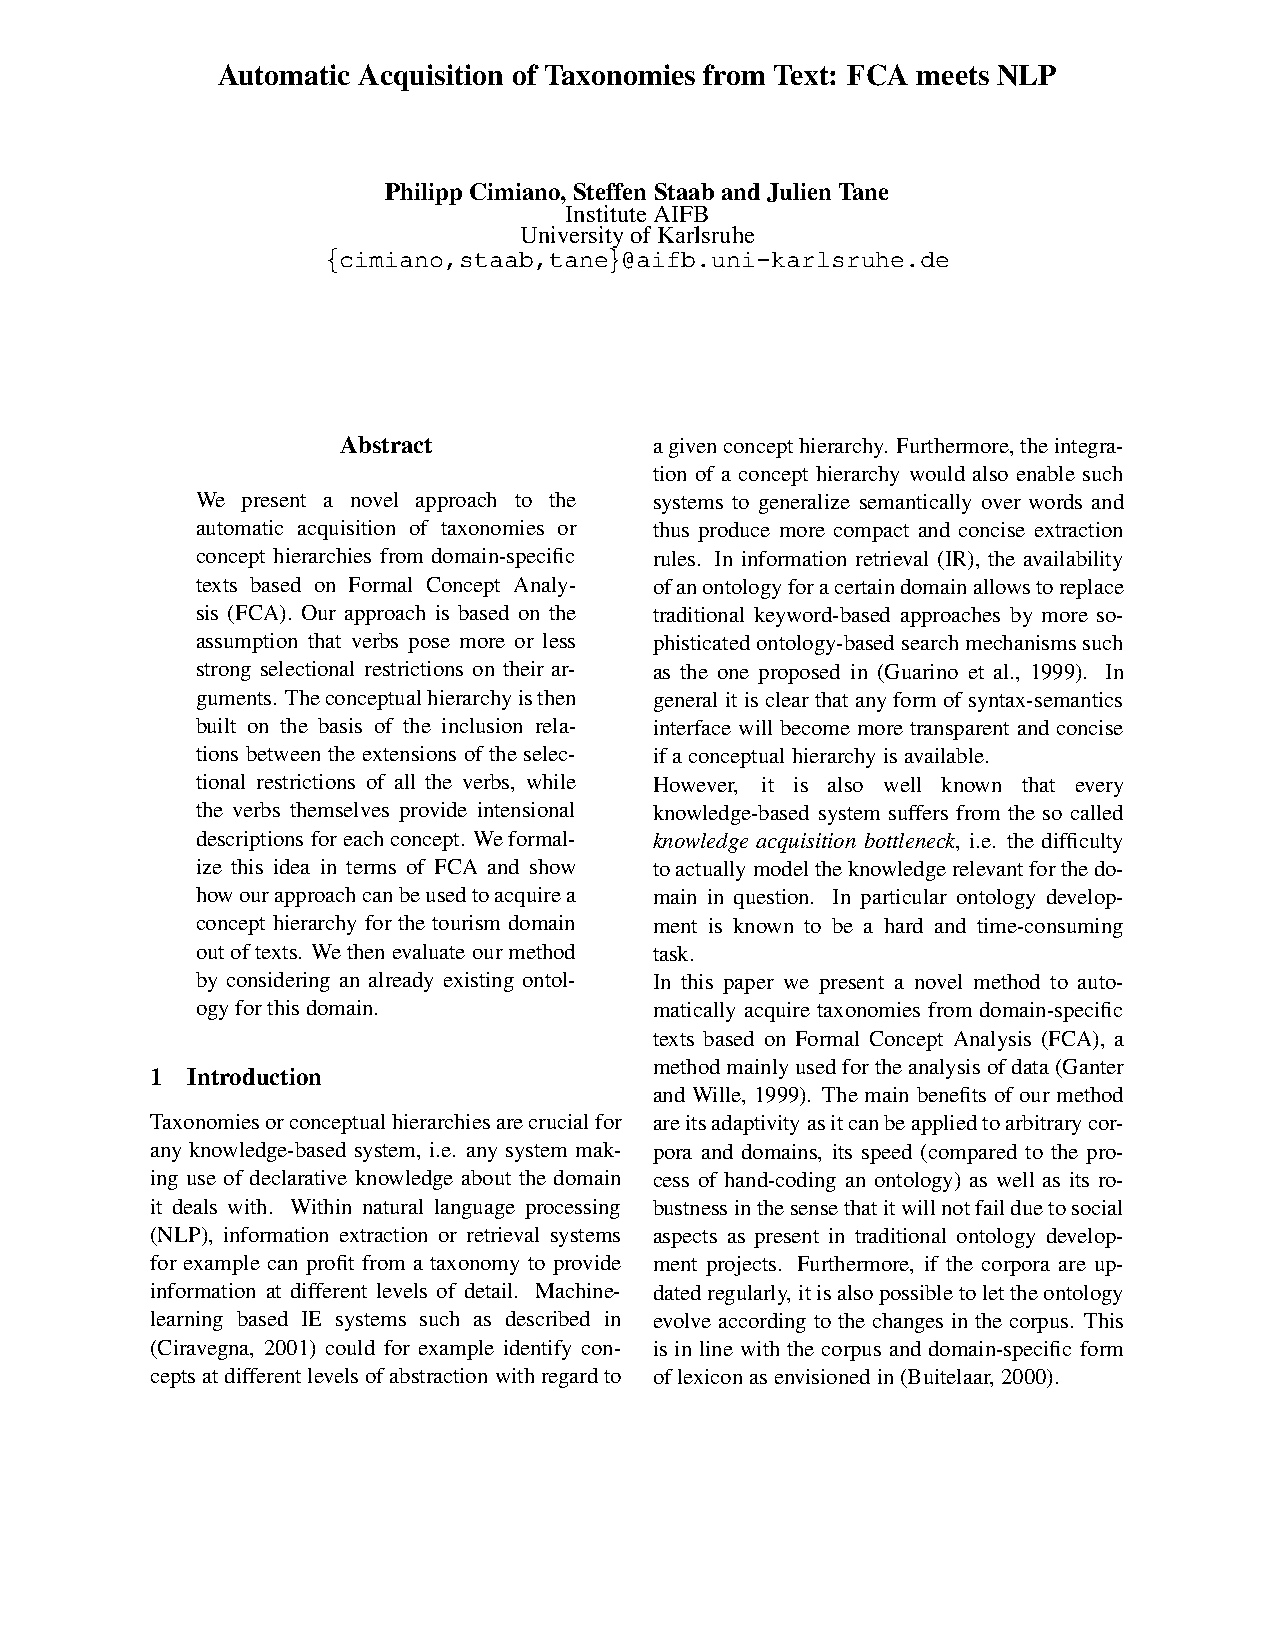
\includepdf[trim= 0 100 0 0,clip=true,offset=0 0,pagecommand={\mbox{}},pages={1-8}]{cimiano-ecml03-atem.pdf}
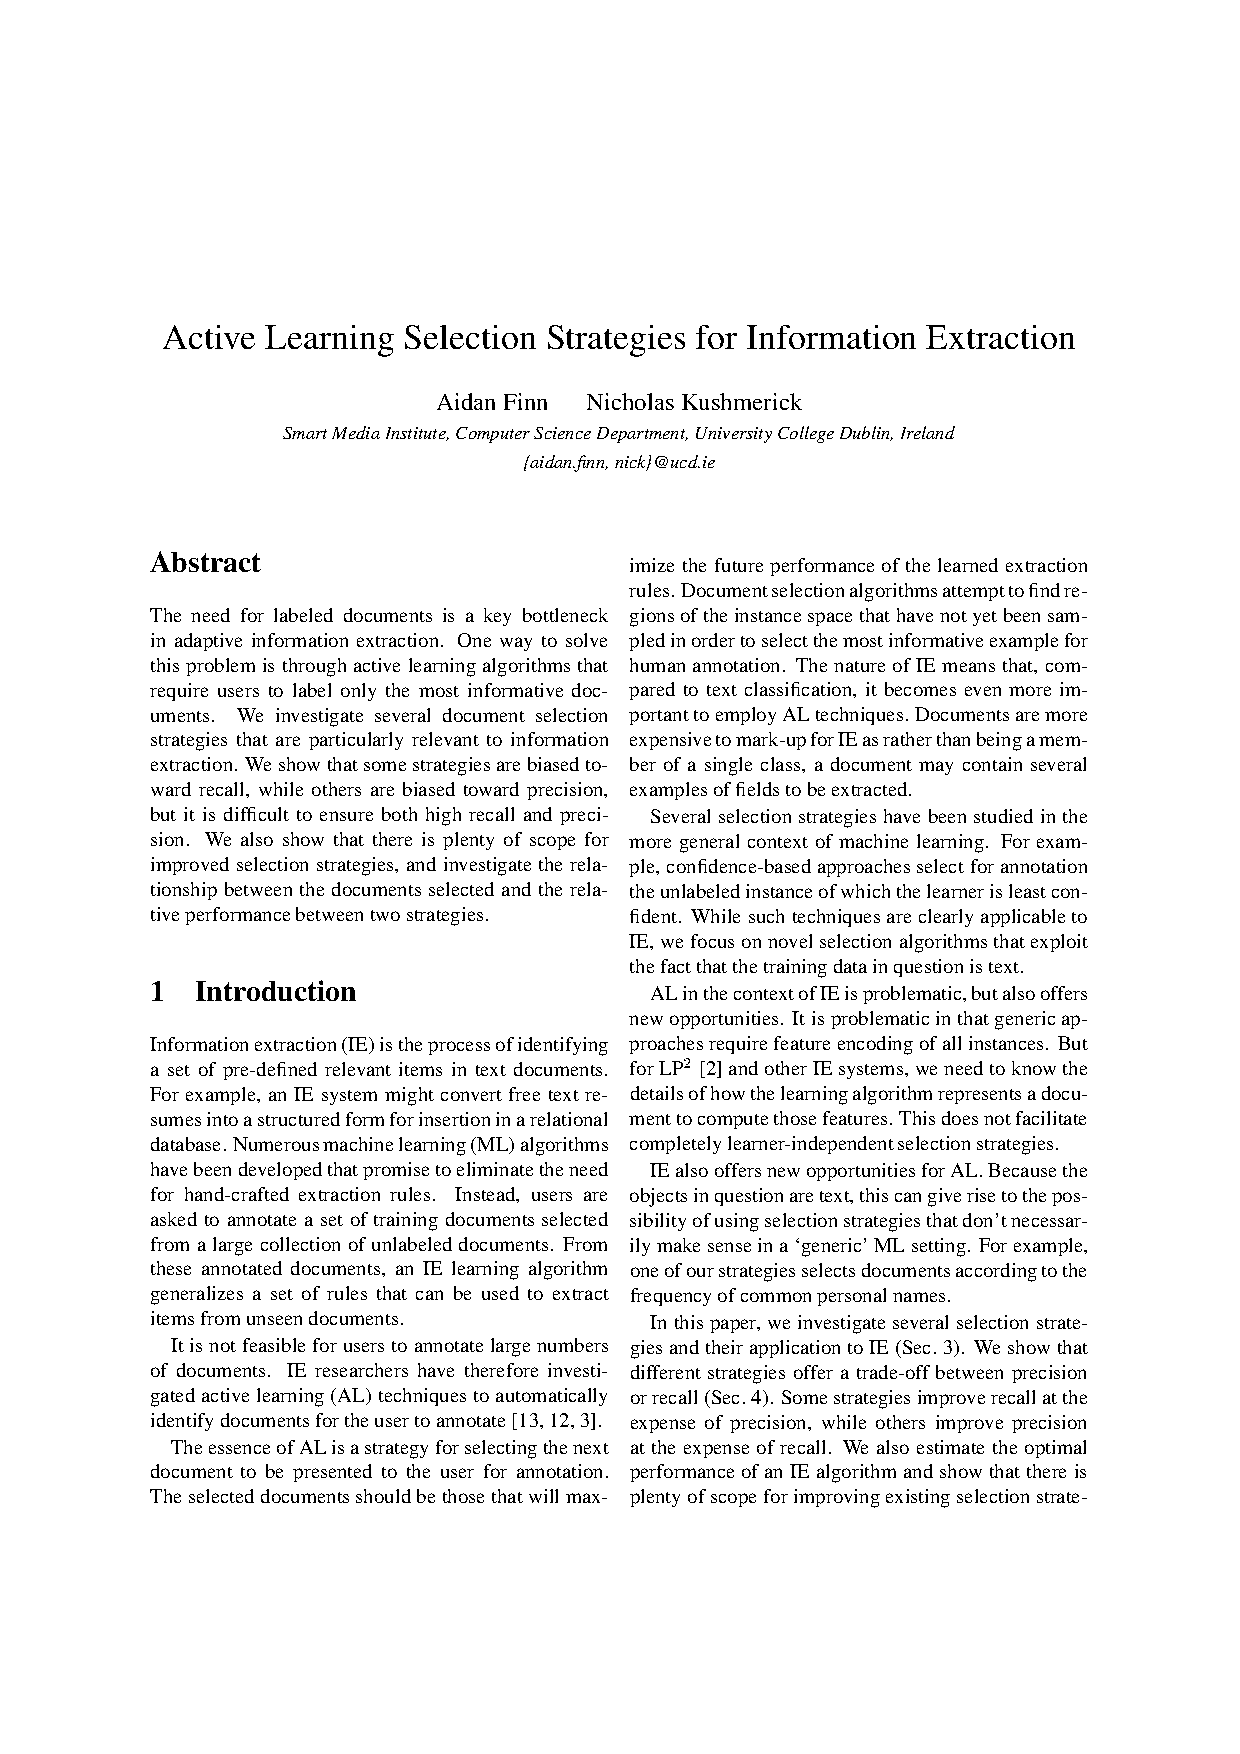
\includepdf[trim= 0 100 0 0,clip=true,offset=0 50,pagecommand={\mbox{}},pages={1-8}]{finn-ecml03-atem.pdf}
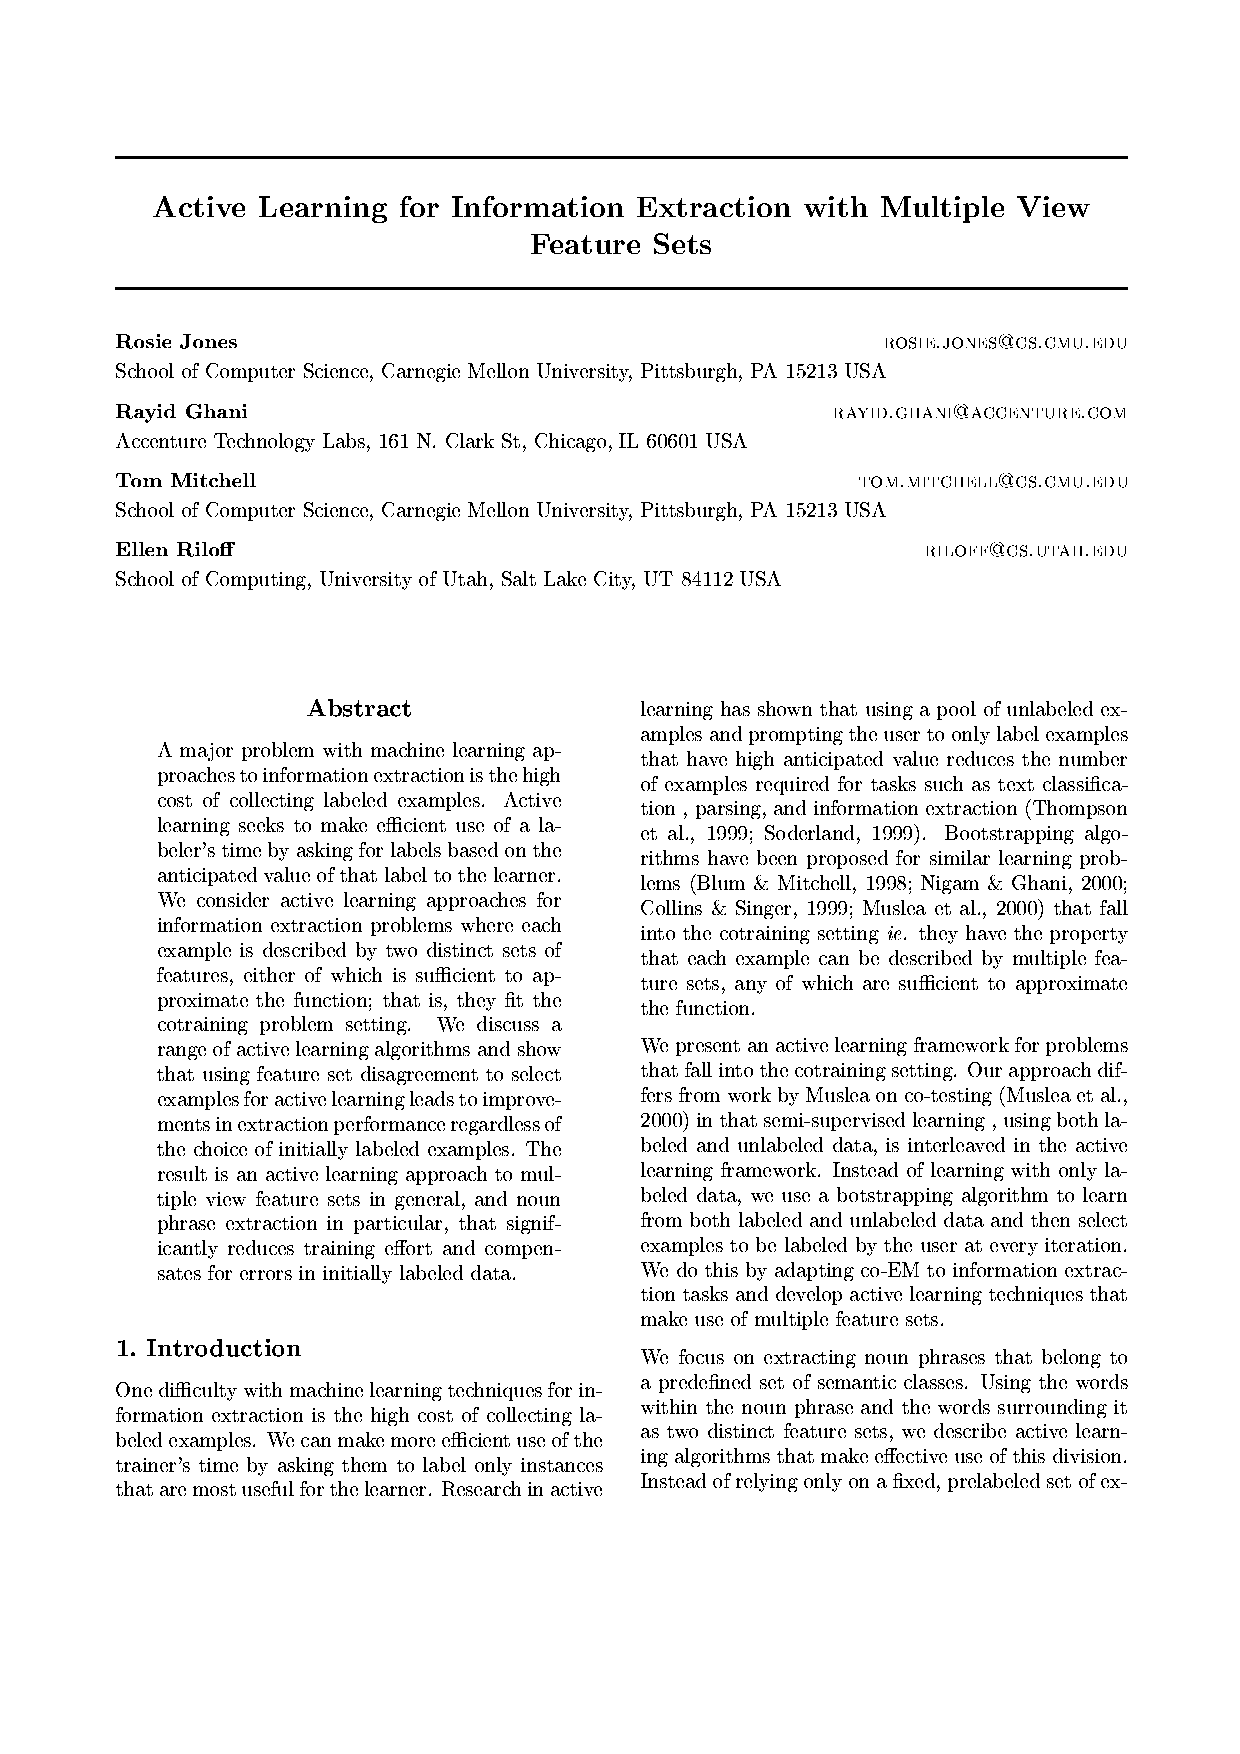
\includepdf[trim= 0 100 0 0,clip=true,offset=0 25,pagecommand={\mbox{}},pages={1-8}]{jones-ecml03-atem.pdf}
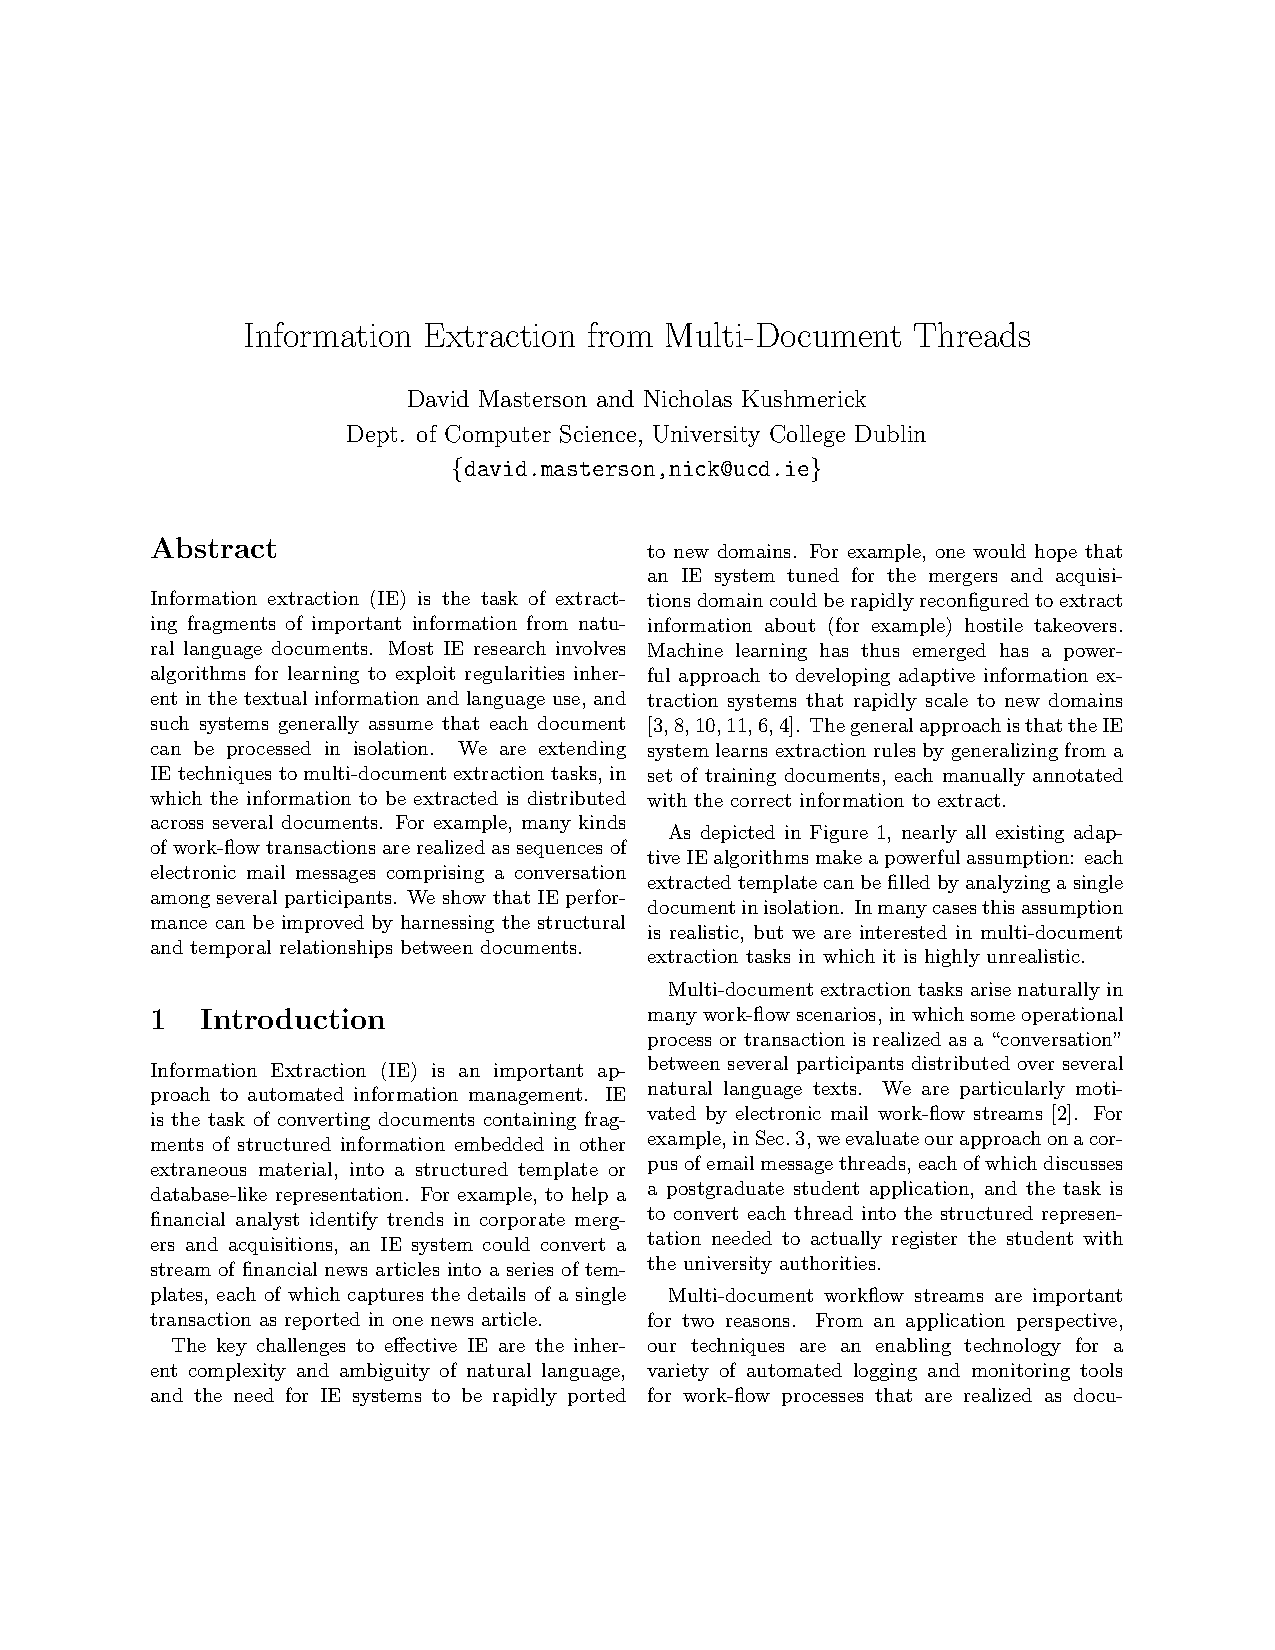
\includepdf[trim= 0 100 0 0,clip=true,offset=0 50,pagecommand={\mbox{}},pages={1-8}]{masterson-ecml03-atem.pdf}
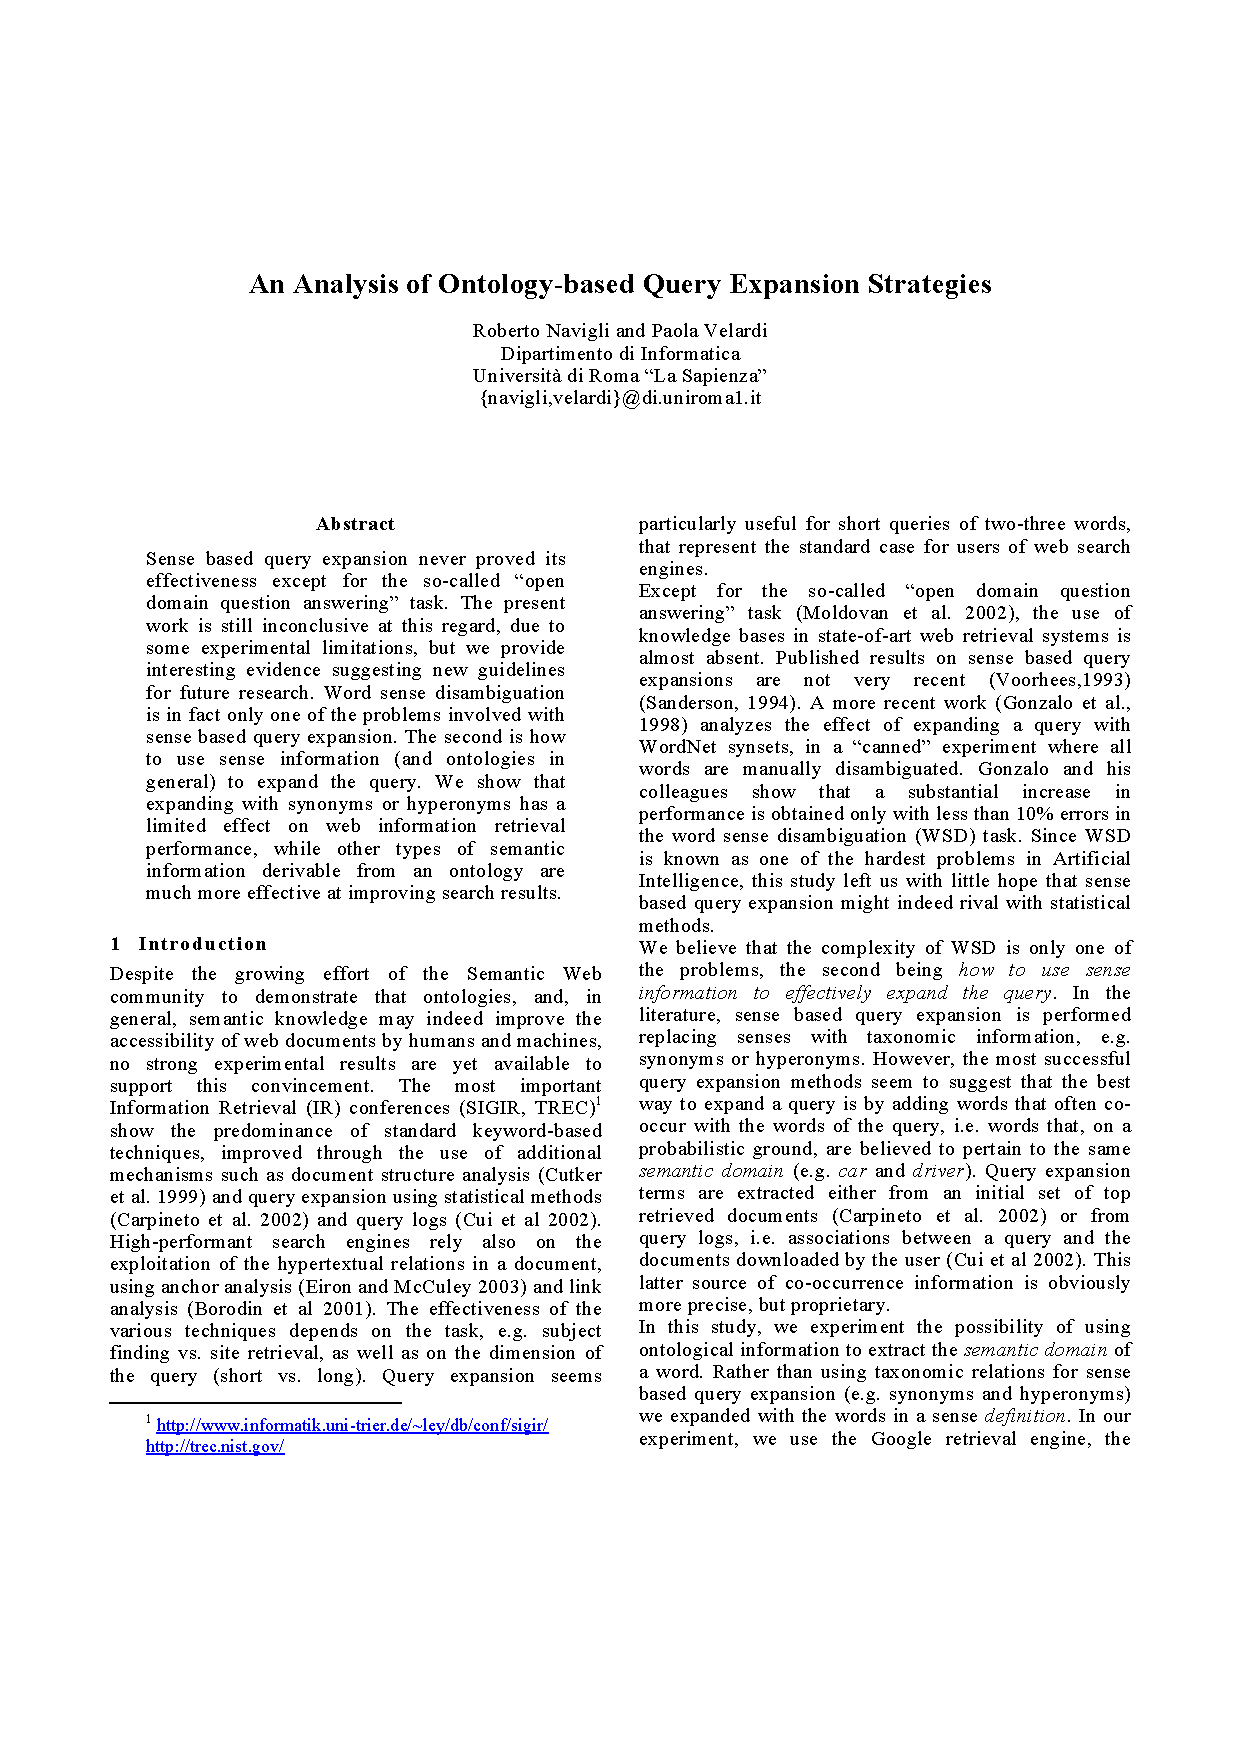
\includepdf[trim= 0 100 0 0,clip=true,offset=0 25,pagecommand={\mbox{}},pages={1-8}]{navigli-ecml03-atem.pdf}
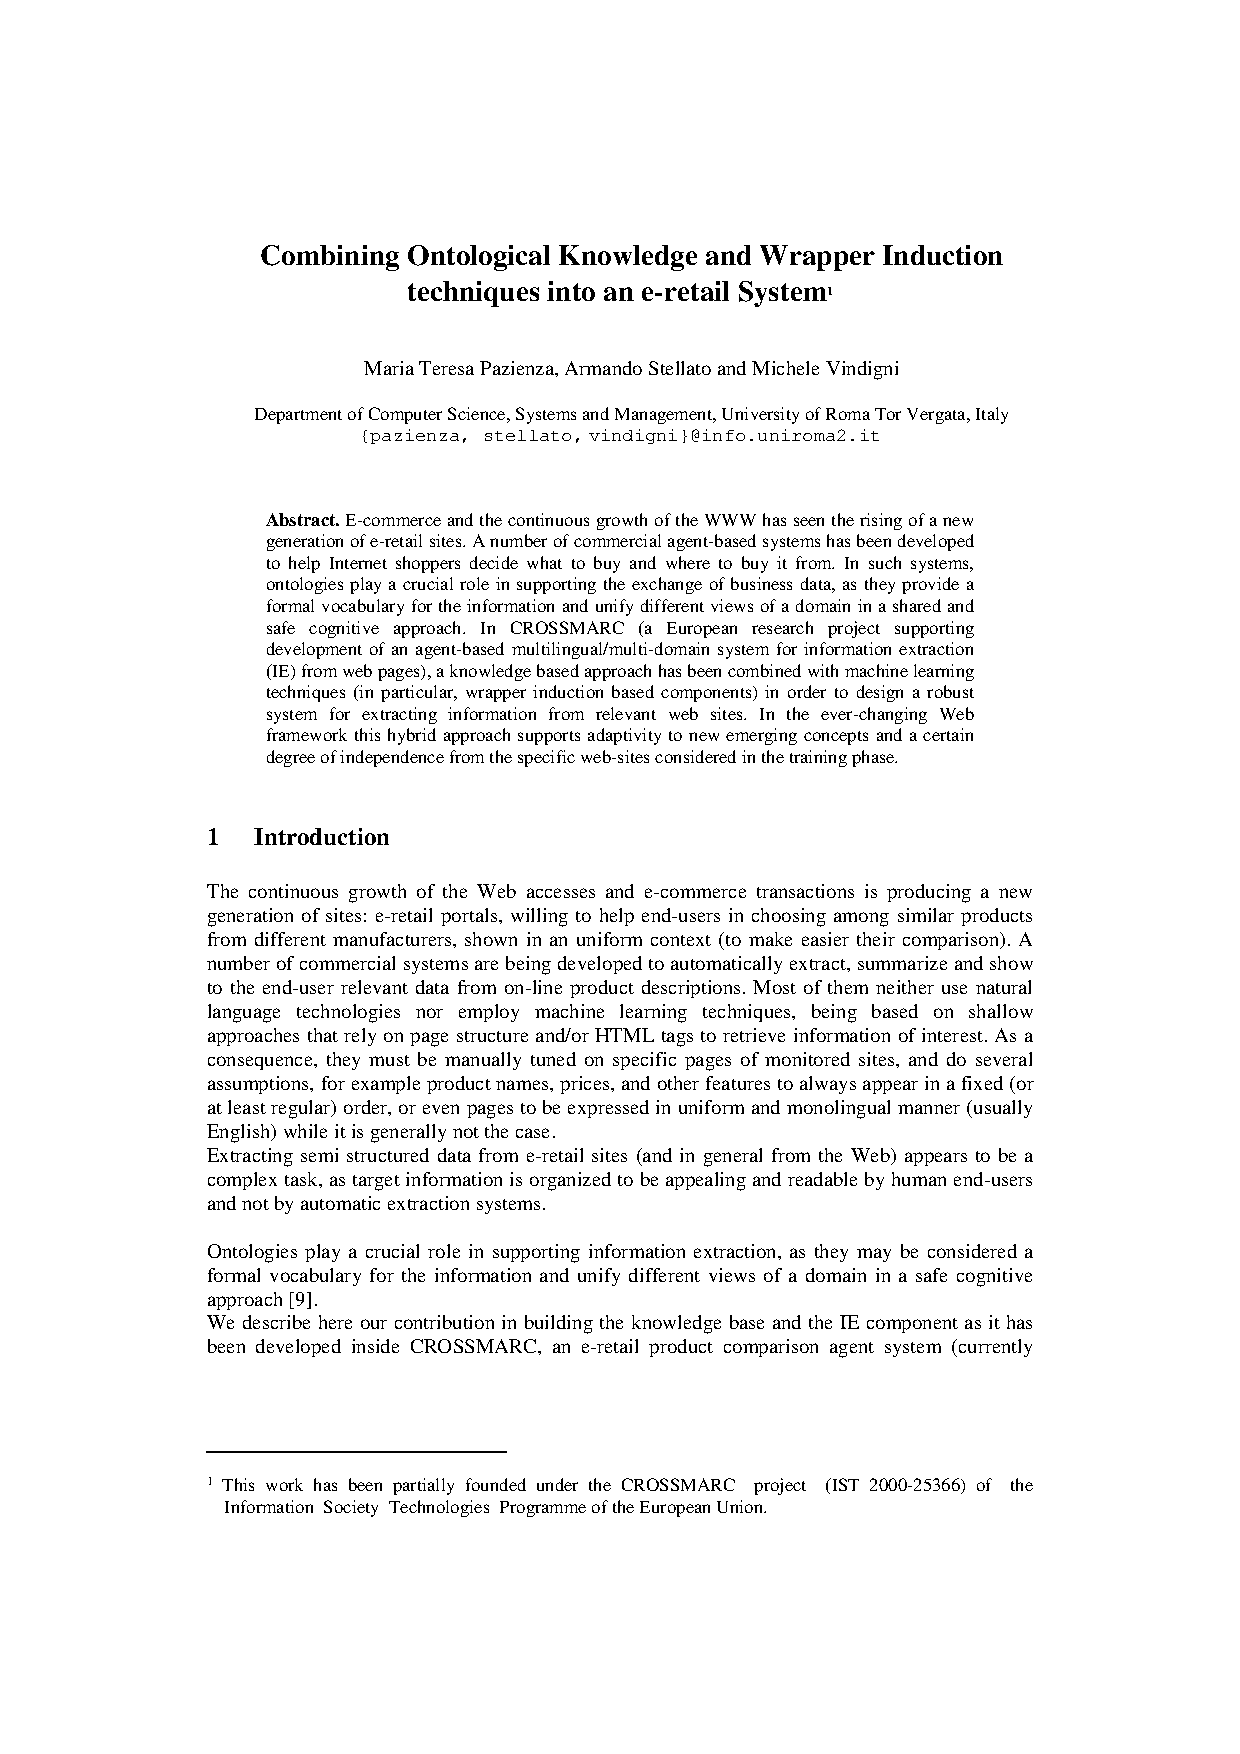
\includepdf[trim= 0 100 0 0,clip=true,offset=0 50,pagecommand={\mbox{}},pages={1-8}]{pazienza-ecml03-atem.pdf}
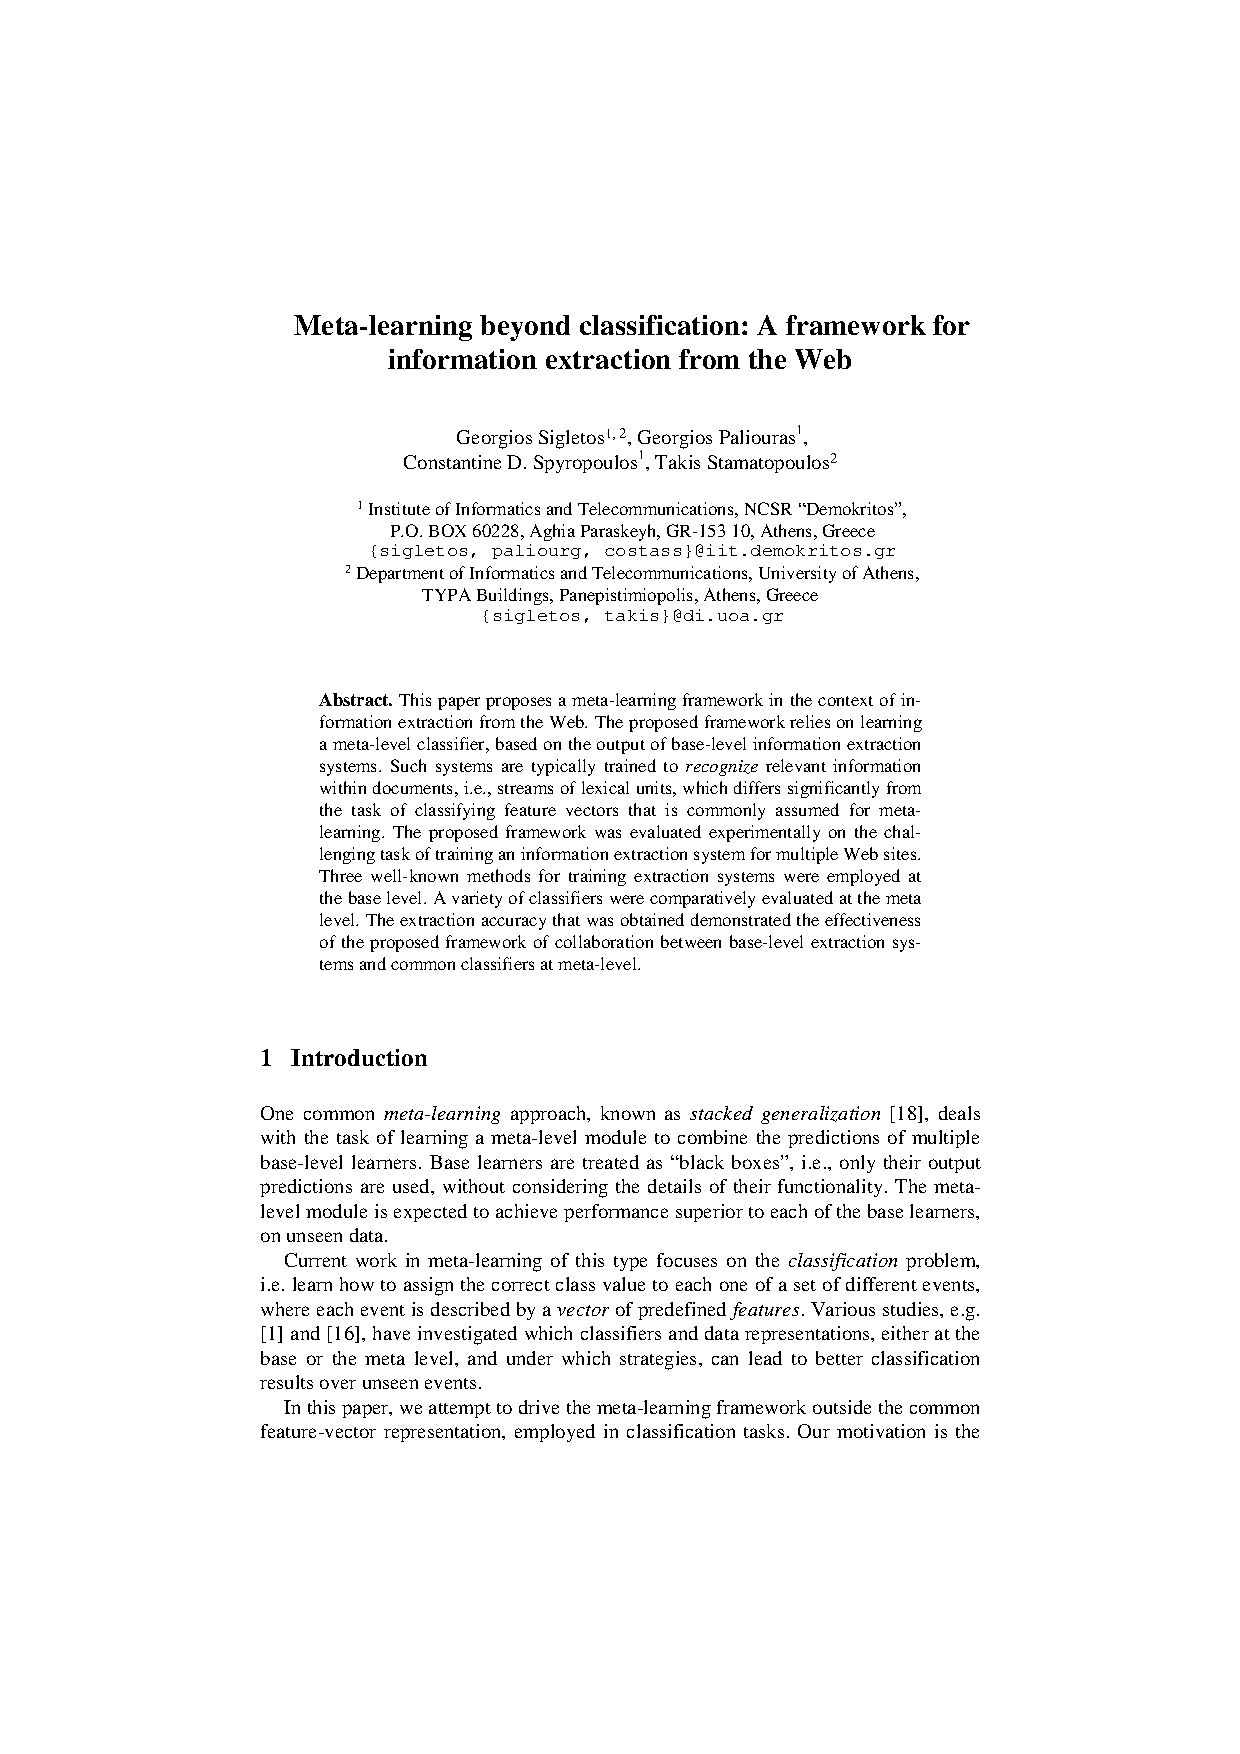
\includepdf[trim= 0 100 0 0,clip=true,offset=0 50,pagecommand={\mbox{}},pages={1-8}]{sigletos-ecml03-atem.pdf}
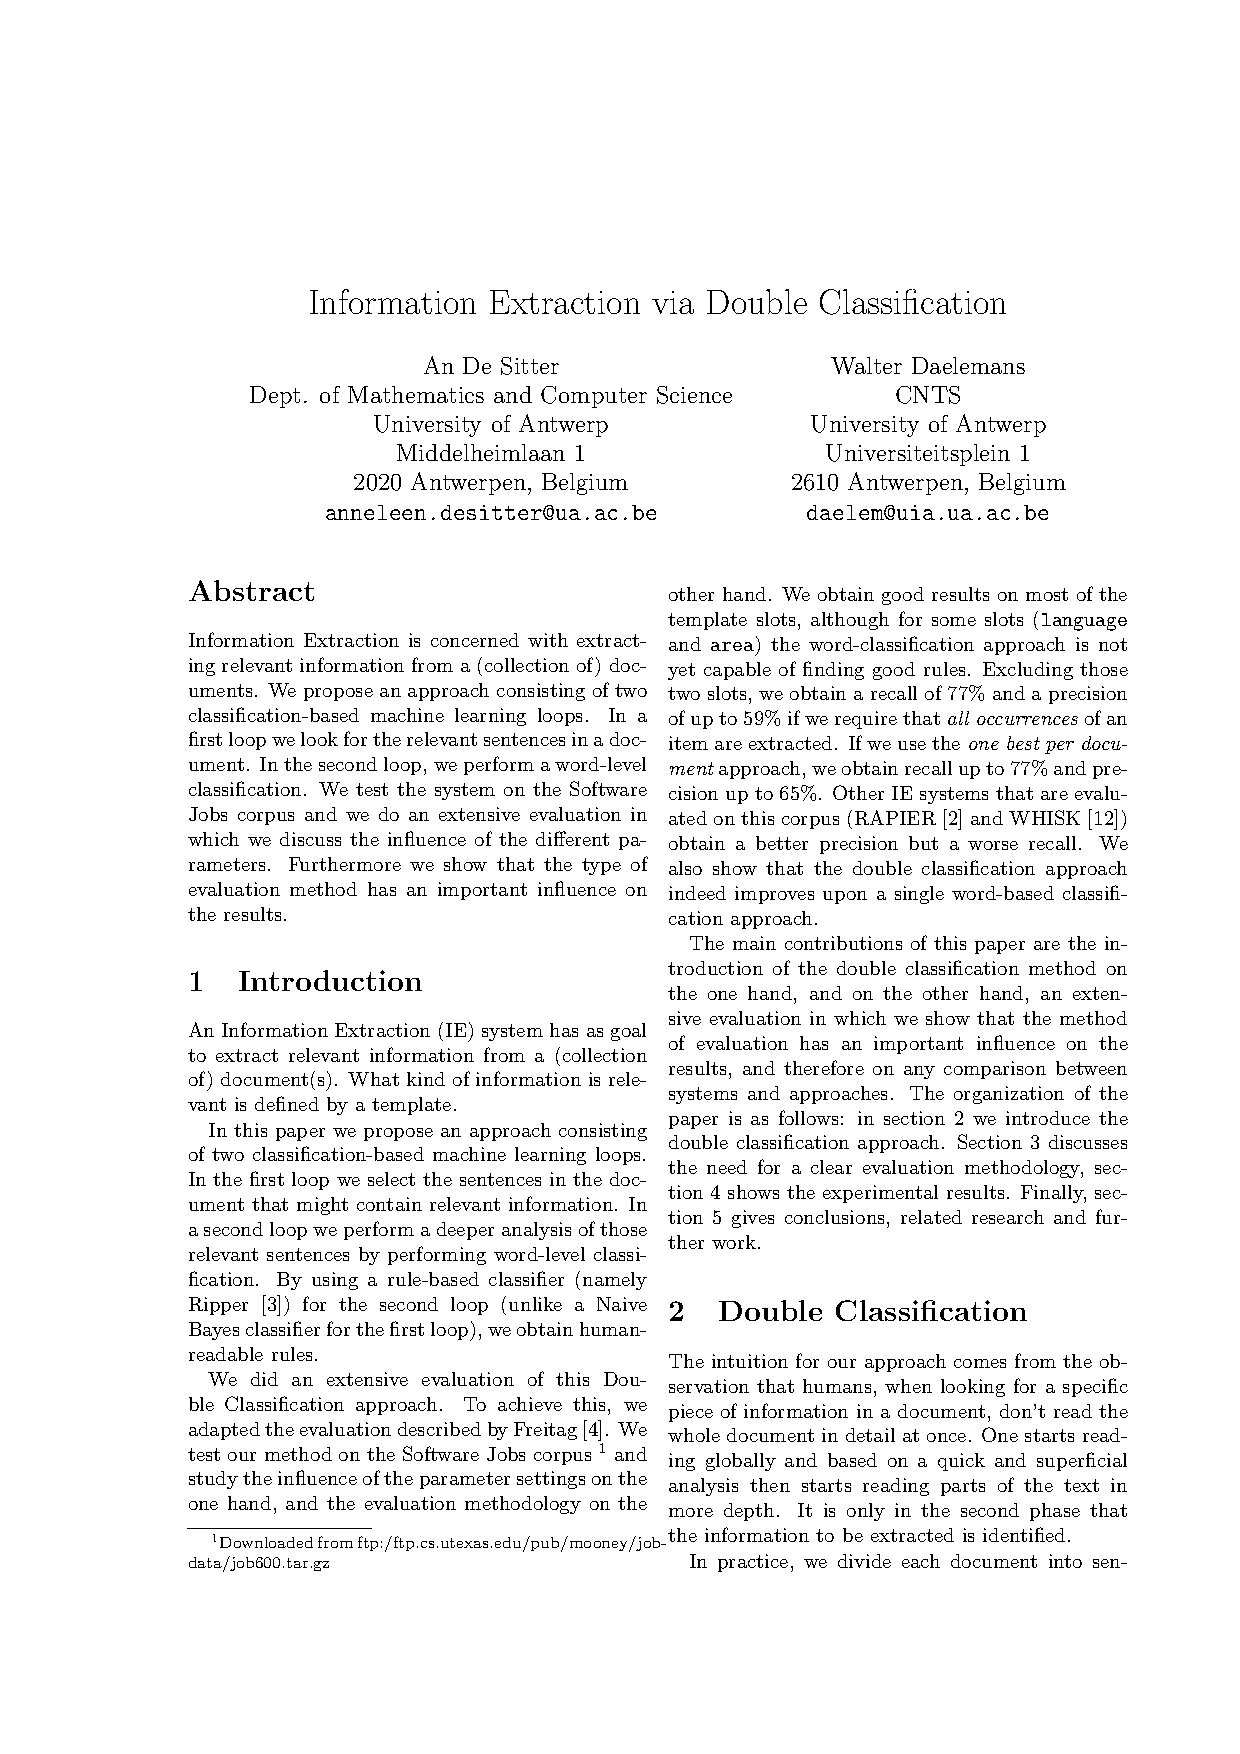
\includepdf[trim= 0 100 0 0,clip=true,offset=-20 50,pagecommand={\mbox{}},pages={1-8}]{desitter-ecml03-atem.pdf}
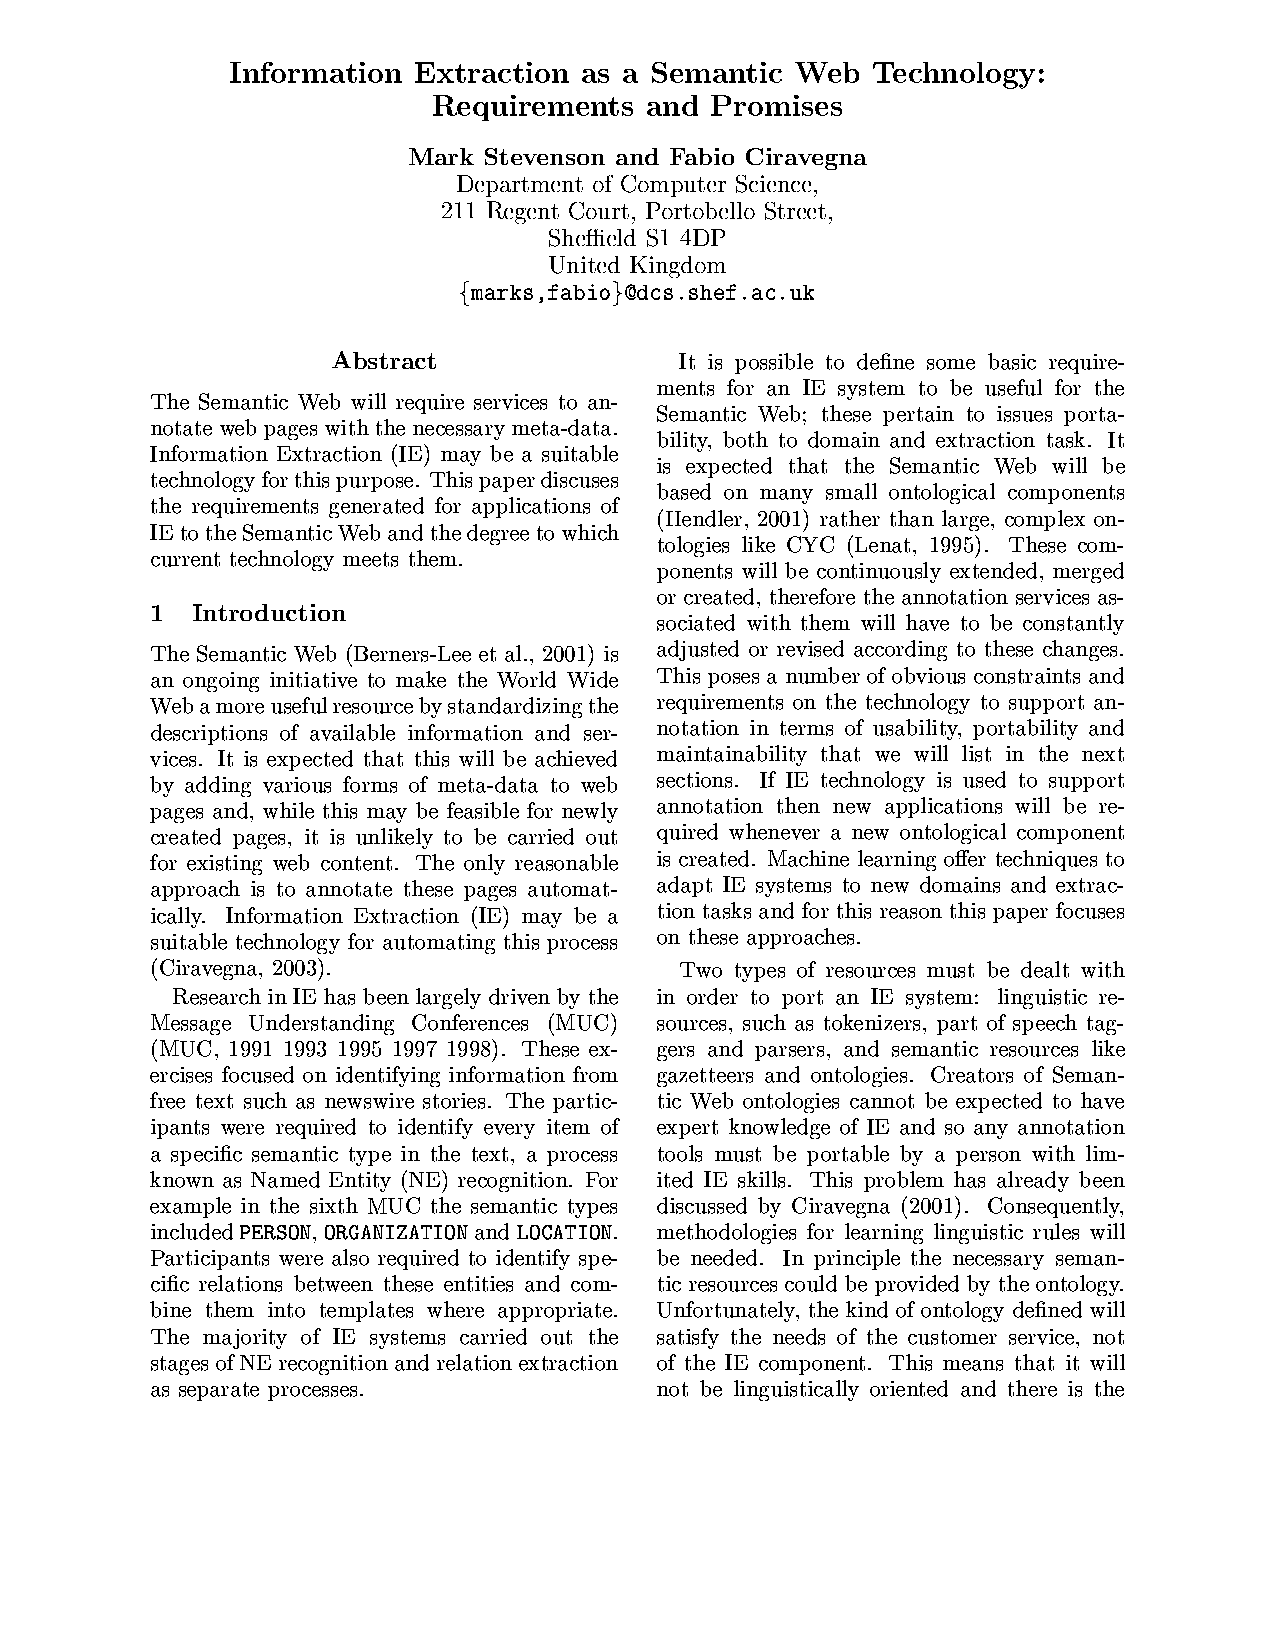
\includepdf[trim= 0 100 0 0,clip=true,offset=0 0,pagecommand={\mbox{}},pages={1-5}]{stevenson-ecml03-atem.pdf}
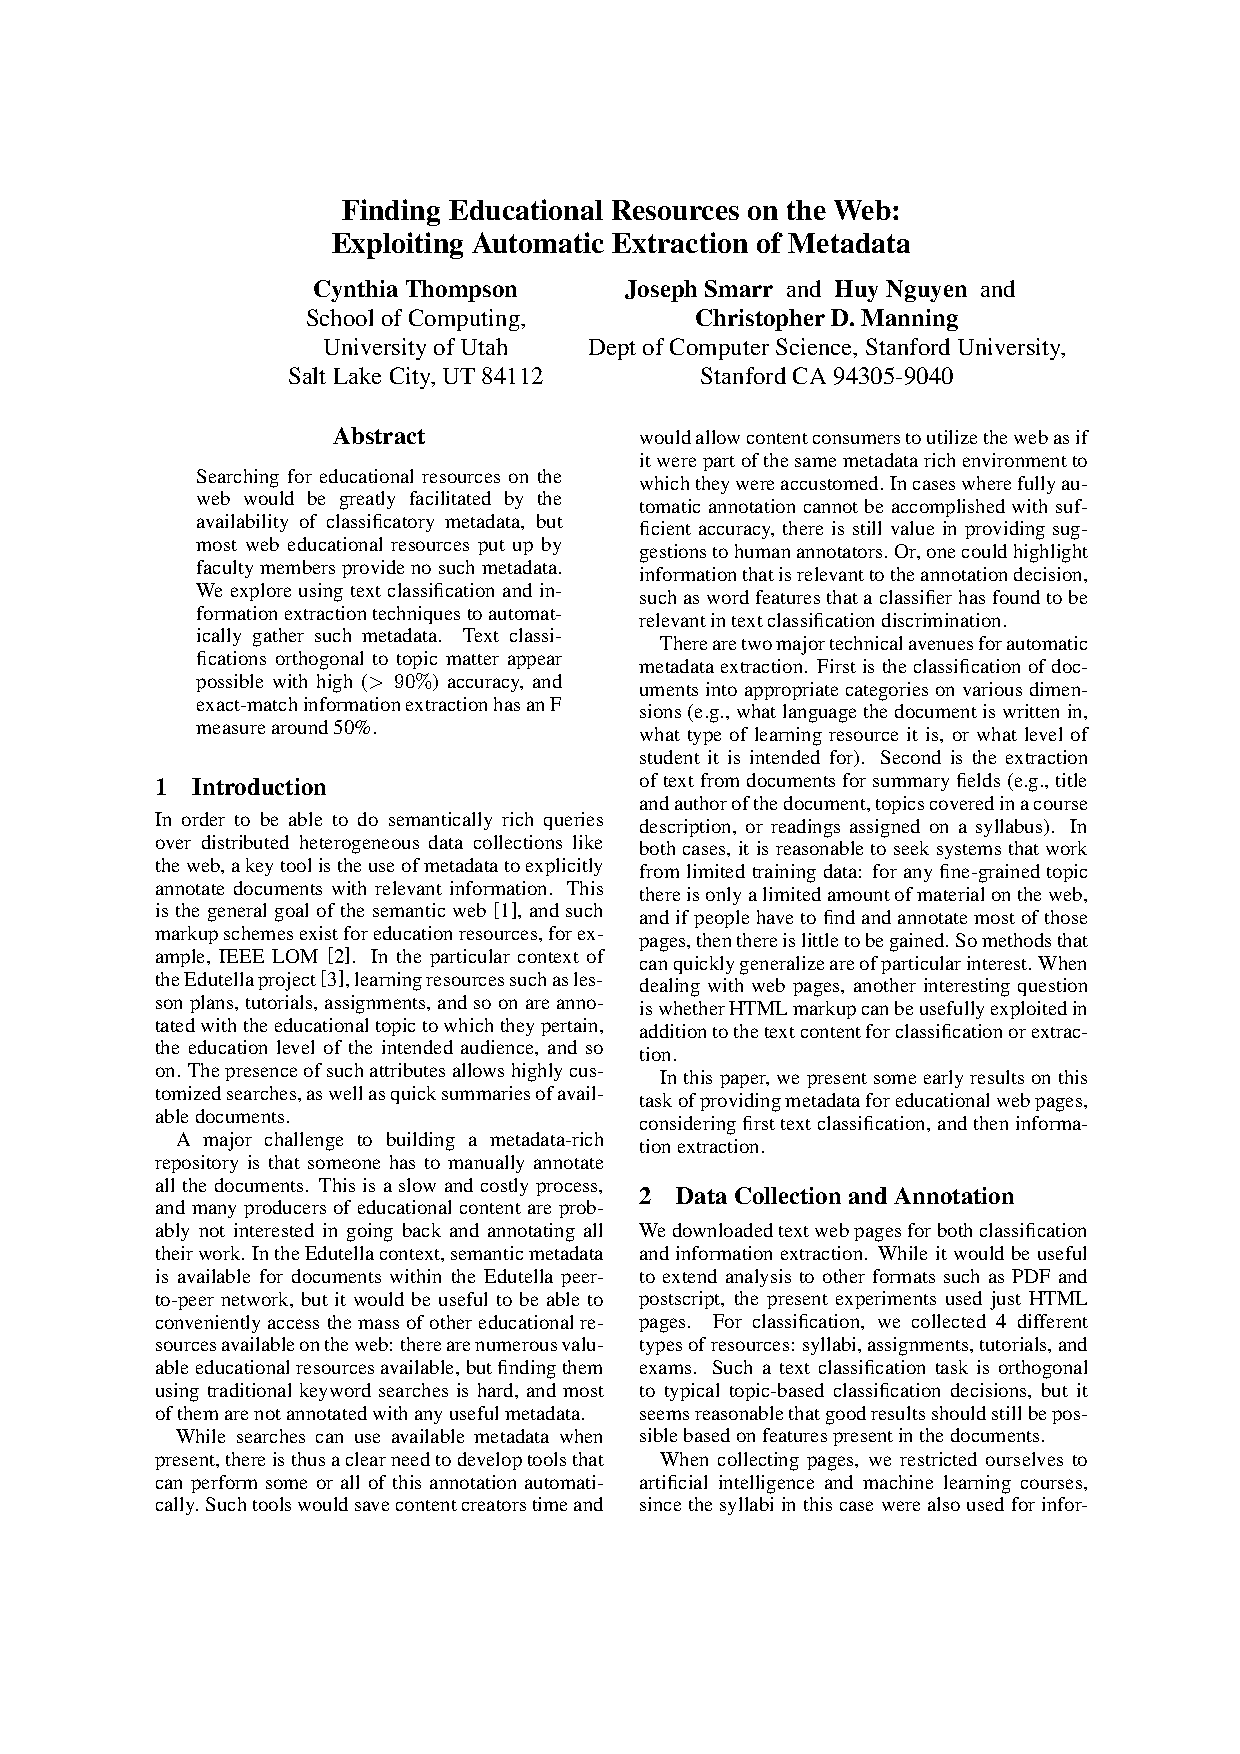
\includepdf[trim= 0 100 0 0,clip=true,offset=0 25,pagecommand={\mbox{}},pages={1-4}]{thompson-ecml03-atem.pdf}
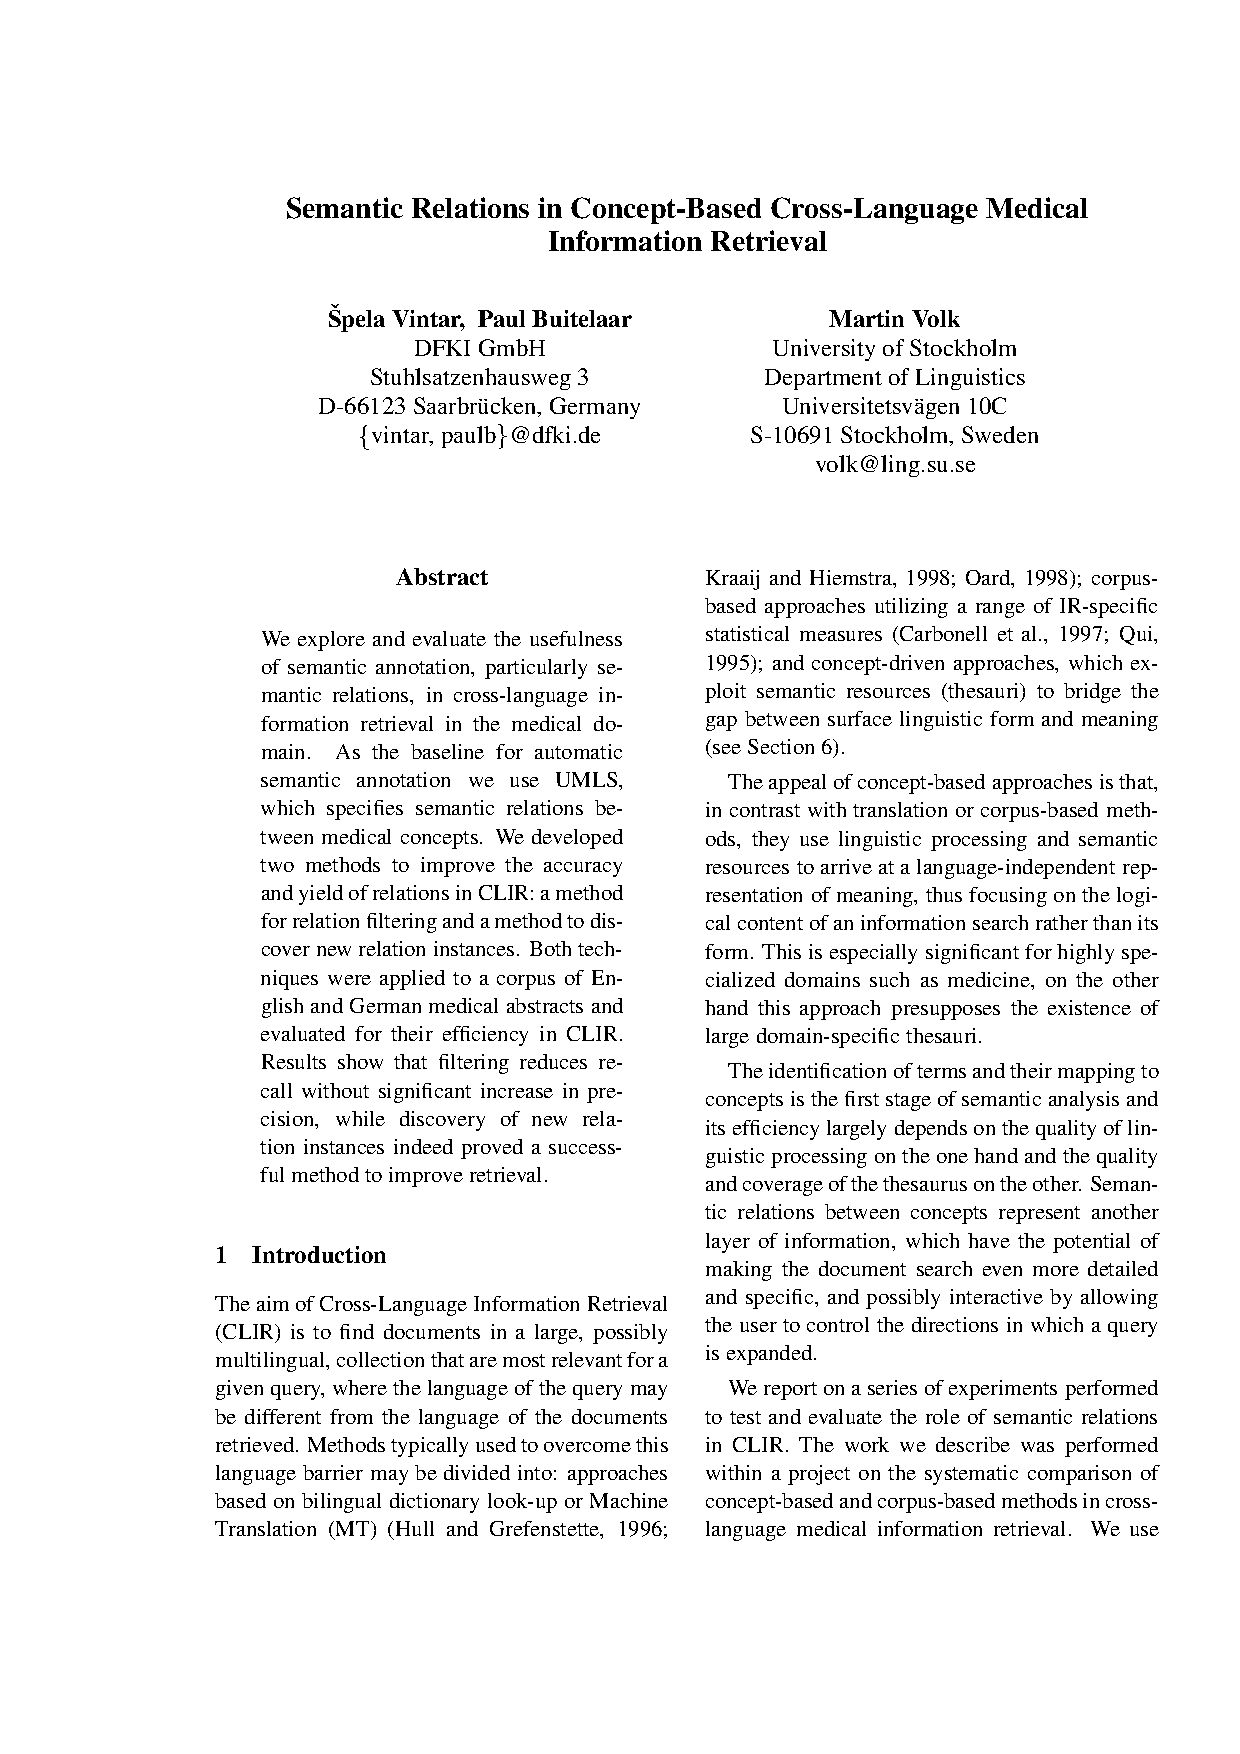
\includepdf[trim= 0 100 0 0,clip=true,offset=-5 50,pagecommand={\mbox{}},pages={1-9}]{vintar-ecml03-atem.pdf}
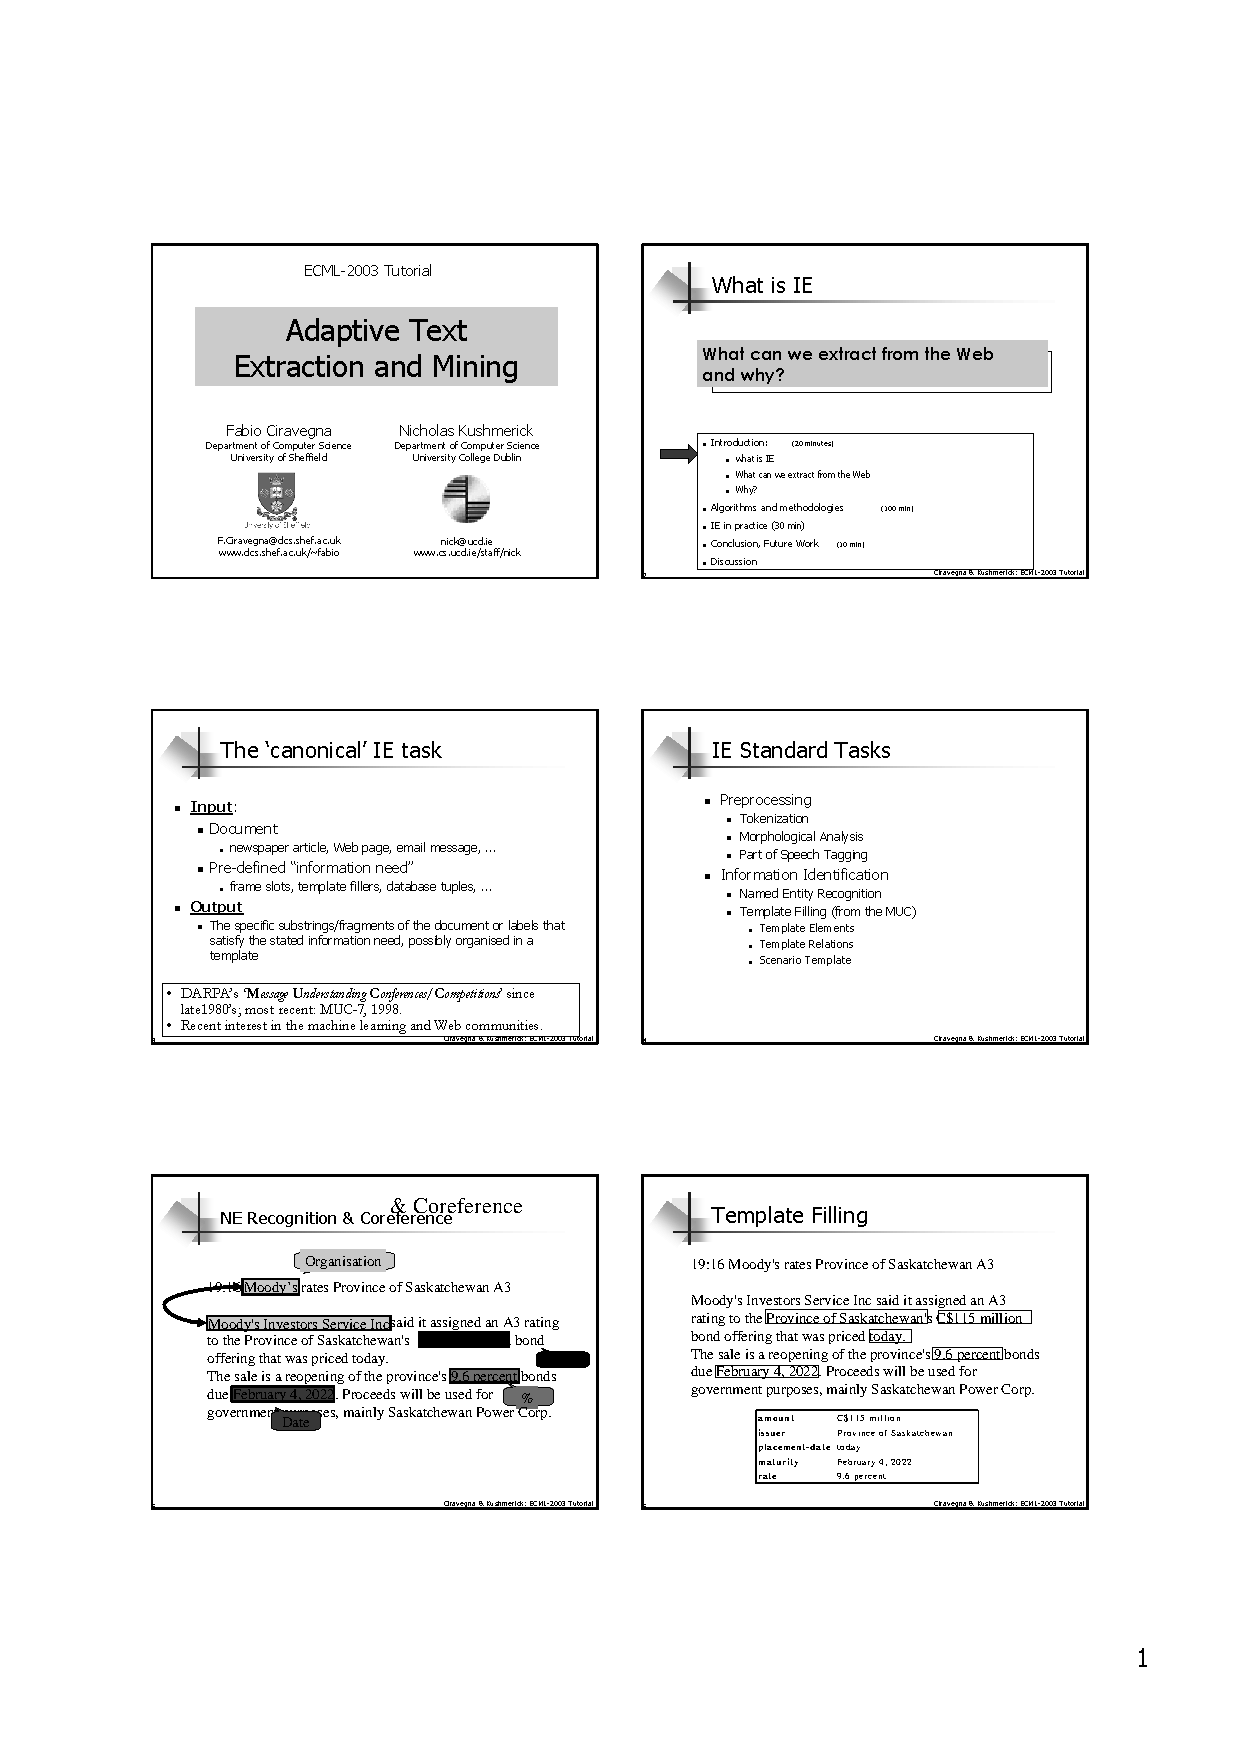
\includepdf[trim= 0 100 0 0,clip=true,offset=0 50,pagecommand={\mbox{}},pages={1-16}]{ECML2003-IE-Tutorial-Ciravegna-Kushmerick-BLACK-AND-WHITE.pdf}

\end{document}
